\documentclass[11pt,a4paper]{article}
\usepackage[T1]{fontenc}
\usepackage[utf8]{inputenc}
\usepackage[french]{babel}
\usepackage{geometry}
\usepackage{graphicx}
\usepackage{booktabs}
\usepackage{listings}
\usepackage{hyperref}
\usepackage{caption}
\usepackage{float}

\geometry{margin=2.3cm}
\hypersetup{colorlinks=true,linkcolor=blue,urlcolor=blue,citecolor=blue}

\lstset{
  basicstyle=\ttfamily\small,
  breaklines=true,
  frame=single,
  numbers=left,
  numberstyle=\tiny,
  tabsize=2,
  language=C++
}

\title{Rapport technique --- Lab 1\\
\large Dépôt \texttt{ns3\_IMT2030\_connectivity}\\
Simulation ns-3, zone dense et gestion heuristique de charge}
\author{Traorehub --- travail de recherche (WIP)}
\date{Novembre 2026}

\begin{document}
\maketitle
\tableofcontents
\newpage

\section{Introduction et objectif du dépôt}

Le dépôt GitHub \texttt{ns3\_IMT2030\_connectivity} organise une recherche sur la connectivité massive et la gestion de charge en zone dense, dans une perspective inspirée du cadre IMT-2030 et de la recommandation ITU-R M.2160. Le simulateur utilisé est ns-3.43, exécuté sous WSL Ubuntu à partir de l'arborescence ns-allinone.

Ce document décrit le Lab 1. Les Labs 2 et 3 sont livrés dans leurs propres rapports. Les Labs 4 et 5 restent au stade du cadrage, dans \texttt{PLANNING.md}. L'objectif du Lab 1 est de montrer une méthodologie reproductible avant d'aborder la couche NR ou les boucles de contrôle de type RAN intelligent.

\section{Honnêteté du modèle radio}

Le Lab 1 ne met pas en oeuvre la pile radio 6G ni le NR 3GPP. Le scénario principal \texttt{imt2030-density-gestion.cc} s'appuie sur Wi-Fi 802.11n dans ns-3. Les éléments techniques effectifs sont les suivants.
\begin{itemize}
  \item \texttt{YansWifiChannelHelper} et \texttt{YansWifiPhyHelper} pour la couche physique ;
  \item \texttt{WIFI\_STANDARD\_80211n} via \texttt{WifiHelper::SetStandard} ;
  \item débit de données fixé à \texttt{HtMcs7} avec contrôle \texttt{HtMcs0} ;
  \item SSID \texttt{imt2030-dense-zone}.
\end{itemize}

Ce choix constitue un \emph{proxy} pédagogique pour une zone dense de type IoT ou mMTC. Il permet de comparer une politique de référence et une politique de gestion tout en reportant l'intégration 5G-LENA au Lab 4. Le nom du dépôt renvoie au cadre de recherche IMT-2030, et non à un simulateur de la stack 6G complète.

\section{Organisation du dépôt et stratégie de travail}

Le dépôt suit une progression en cinq laboratoires sous \texttt{labs/}. Le Lab 1 regroupe le scénario C++, les scripts de figures, les sorties CSV et les captures d'écran. Les fichiers \texttt{docs/CADRE\_IMT2030.md} et \texttt{PLANNING.md} fixent les hypothèses et la feuille de route.

La stratégie retenue consiste à séparer clairement la vision IMT (densité extrême, gestion intelligente) du modèle simulable (grille de terminaux, un point d'accès, trafic UDP). Chaque campagne conserve les mêmes paramètres géométriques et ne change que la politique \texttt{baseline} ou \texttt{adaptive}, afin de respecter un protocole expérimental simple.

\section{Méthodologie du Lab 1}

\subsection{Topologie et trafic}

Le nombre de terminaux vaut $N = \texttt{gridSide}^2$. Les positions suivent un \texttt{GridPositionAllocator} avec espacement 5~m. Le point d'accès est placé au-dessus du centre de la grille. Chaque terminal exécute une application \texttt{UdpClient} vers le \texttt{PacketSink} installé sur le point d'accès.

\subsection{Politique baseline}

En mode \texttt{baseline}, tous les clients émettent selon \texttt{packetsPerSta}, \texttt{intervalMs} et \texttt{packetSize} sans intervention du contrôleur.

\subsection{Politique adaptive (version 0)}

Toutes les 0,5~s, le contrôleur estime le rapport
\[
  \rho = \frac{\text{débit offert par les terminaux actifs}}{\text{capacité de référence}}
\]
où la capacité de référence vaut 8~Mbit/s par défaut (\texttt{capacityMbps}). Si $\rho > 0{,}82$, environ un quart des terminaux encore actifs est mis en veille via \texttt{ApplicationContainer::Stop}. Si $\rho < 0{,}55$ et si des terminaux sont en veille, un terminal est réactivé. Cette logique s'inspire d'une admission simplifiée sous saturation, sans équivalent direct d'un near-RT RIC.

\subsection{Métriques enregistrées}

À la fin de la simulation, le programme affiche et append dans \texttt{sorties/resultats.csv} les grandeurs suivantes.
\begin{itemize}
  \item \texttt{bytesRx} : octets reçus au point d'accès ;
  \item \texttt{bytesOfferedEst} : estimation de l'offre (paquets prévus fois taille) ;
  \item \texttt{deliveryRatio} : quotient des deux ;
  \item \texttt{throttleEvents} : nombre d'actions Stop ou Start ;
  \item \texttt{jainFairness} : indice de Jain sur les octets reçus par flux FlowMonitor.
\end{itemize}

Ces définitions décrivent la version 0 du scénario. Le rapport du Lab 3, dans la section « Lecture concrète des métriques », indique comment lire les mêmes colonnes après le changement d'émetteur, avec un exemple en nombre de paquets.

\section{Extraits de code stratégiques}

\subsection{Paramètres globaux du contrôleur}

\begin{lstlisting}
static double g_highUtil = 0.82;
static double g_lowUtil = 0.55;
static uint64_t g_capacityBps = 8000000;
static Time g_measureWindow = Seconds(0.5);
\end{lstlisting}

\subsection{Boucle adaptive}

\begin{lstlisting}
const double offeredBps = activeCount * (pktBits / intervalSec);
const double rho = offeredBps / static_cast<double>(g_capacityBps);
if (rho > g_highUtil) {
  // mise en veille d'environ 25 % des STA actifs
  ThrottleSta(s, true);
} else if (rho < g_lowUtil && throttledCount > 0) {
  ThrottleSta(s, false);
}
\end{lstlisting}

\subsection{Stack Wi-Fi effective}

\begin{lstlisting}
wifi.SetStandard(WIFI_STANDARD_80211n);
wifi.SetRemoteStationManager("ns3::ConstantRateWifiManager",
    "DataMode", StringValue("HtMcs7"),
    "ControlMode", StringValue("HtMcs0"));
Ssid ssid("imt2030-dense-zone");
\end{lstlisting}

\section{Résultats des campagnes effectuées}

Le tableau~\ref{tab:resultats} synthétise les principales exécutions consignées dans \texttt{resultats.csv}. Les lignes dupliquées correspondent à des relances de la même configuration.

\begin{table}[H]
  \centering
  \caption{Synthèse des runs enregistrés (extrait de \texttt{resultats.csv})}
  \label{tab:resultats}
  \small
  \begin{tabular}{@{}llrrrrr@{}}
    \toprule
    Grille & Politique & $T$ (s) & Livraison & Jain & Throttle & Octets RX \\
    \midrule
    6$\times$6 (36 STA) & baseline & 10 & 0,967 & 0,992 & 0 & 713\,216 \\
    6$\times$6 (36 STA) & adaptive & 10 & 0,967 & 0,992 & 0 & 713\,216 \\
    8$\times$8 (64 STA) & baseline & 15 & 0,567 & 0,939 & 0 & 742\,912 \\
    8$\times$8 (64 STA) & adaptive & 15 & 0,567 & 0,939 & 0 & 742\,912 \\
    10$\times$10 (100 STA) & baseline & 12 & 0,186 & 0,851 & 0 & 381\,440 \\
    10$\times$10 (100 STA) & adaptive & 12 & 0,186 & 0,851 & 50 & 381\,440 \\
    \bottomrule
  \end{tabular}
\end{table}

\subsection{Interprétation}

Pour la grille 6$\times$6 à charge modérée, baseline et adaptive coïncident car l'offre agrégée reste sous le seuil haut du contrôleur. Aucun événement \texttt{throttle} n'apparaît.

Pour la grille 8$\times$8 avec durée 15~s et intervalle par défaut (80~ms), le taux de livraison est d'environ 57~\%. Le contrôleur ne s'active toujours pas, ce qui confirme que la saturation observée provient surtout du canal Wi-Fi et non de la politique adaptive.

Pour la grille 10$\times$10 avec \texttt{intervalMs=40}, la livraison tombe à environ 18,6~\%. La politique adaptive déclenche 50 événements de gestion alors que la baseline n'en déclenche aucun. Sur cette version du contrôleur, le débit utile mesuré à l'AP reste identique entre les deux politiques. La prochaine itération (Lab 3) devra faire évoluer la livraison effective, et pas seulement le compteur d'actions.

\section{Figures du Lab 1}

Les figures suivantes sont versionnées dans le dépôt. Elles peuvent être régénérées avec \texttt{scripts/generer\_toutes\_les\_images.py}.

Les vues vectorielles \texttt{image\_topologie.svg} et \texttt{image\_comparatif.svg} se trouvent dans \texttt{labs/lab01\_wifi\_dense/sorties/}. Le format PDF standard ne les intègre pas toujours sans conversion. Les captures terminal ci-dessous proviennent des campagnes réelles.

\begin{figure}[H]
  \centering
  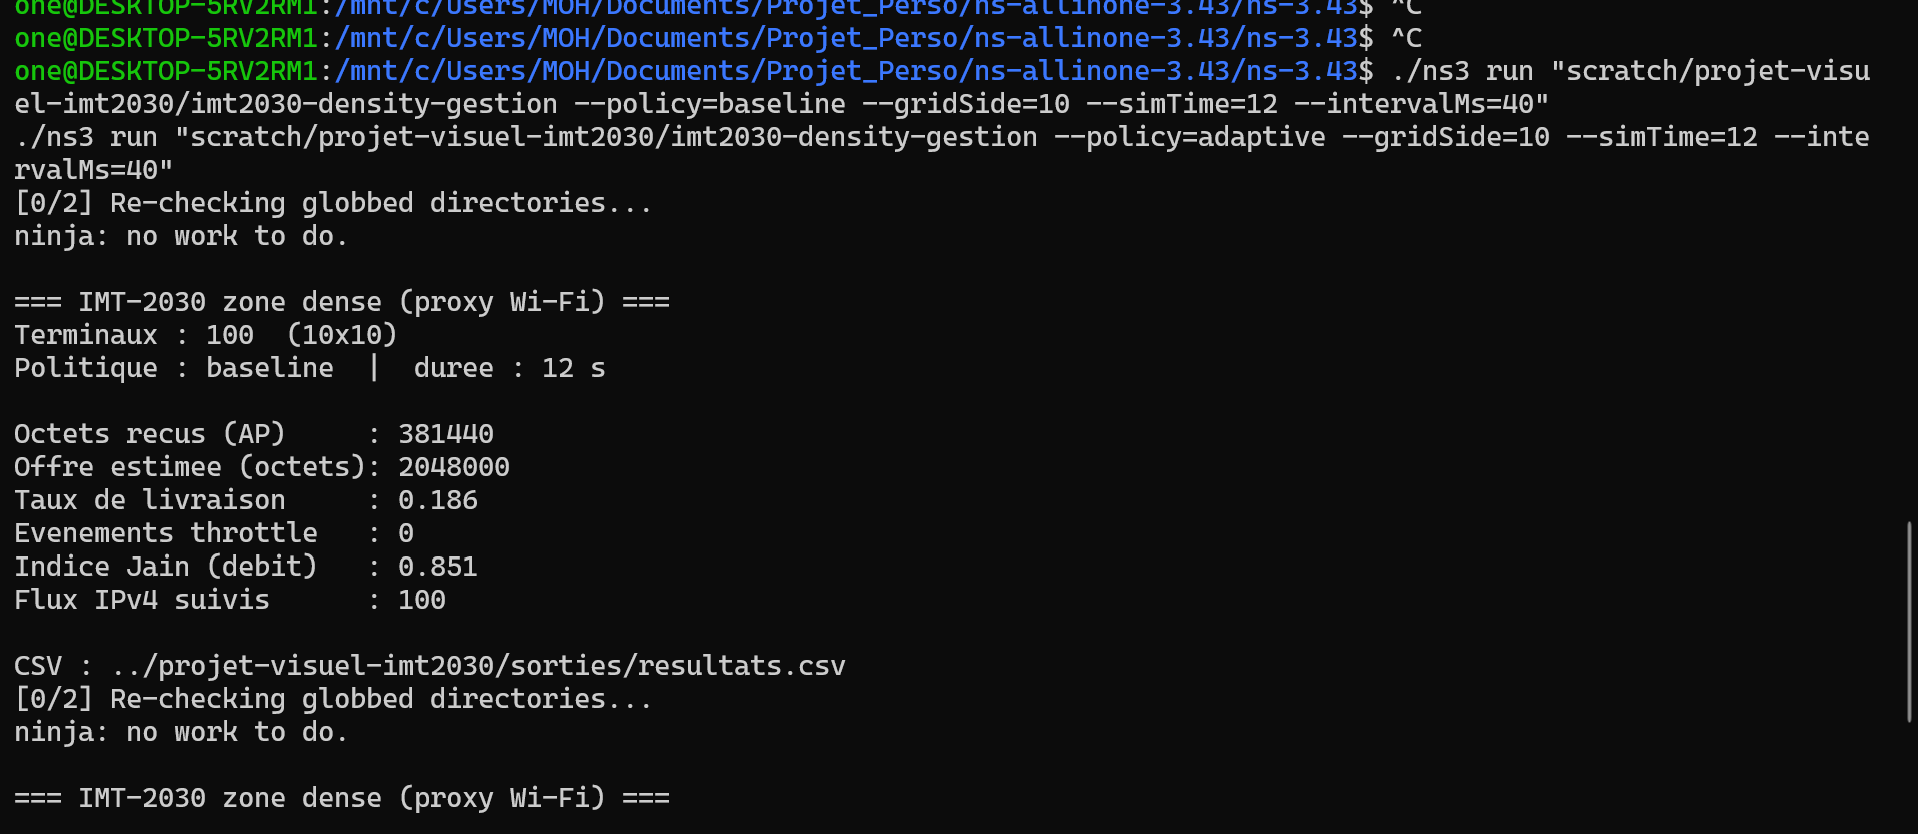
\includegraphics[width=0.95\linewidth]{../../labs/lab01_wifi_dense/docs/img/terminal-baseline-10x10.png}
  \caption{Sortie terminal : campagne 10$\times$10, politique baseline.}
\end{figure}

\begin{figure}[H]
  \centering
  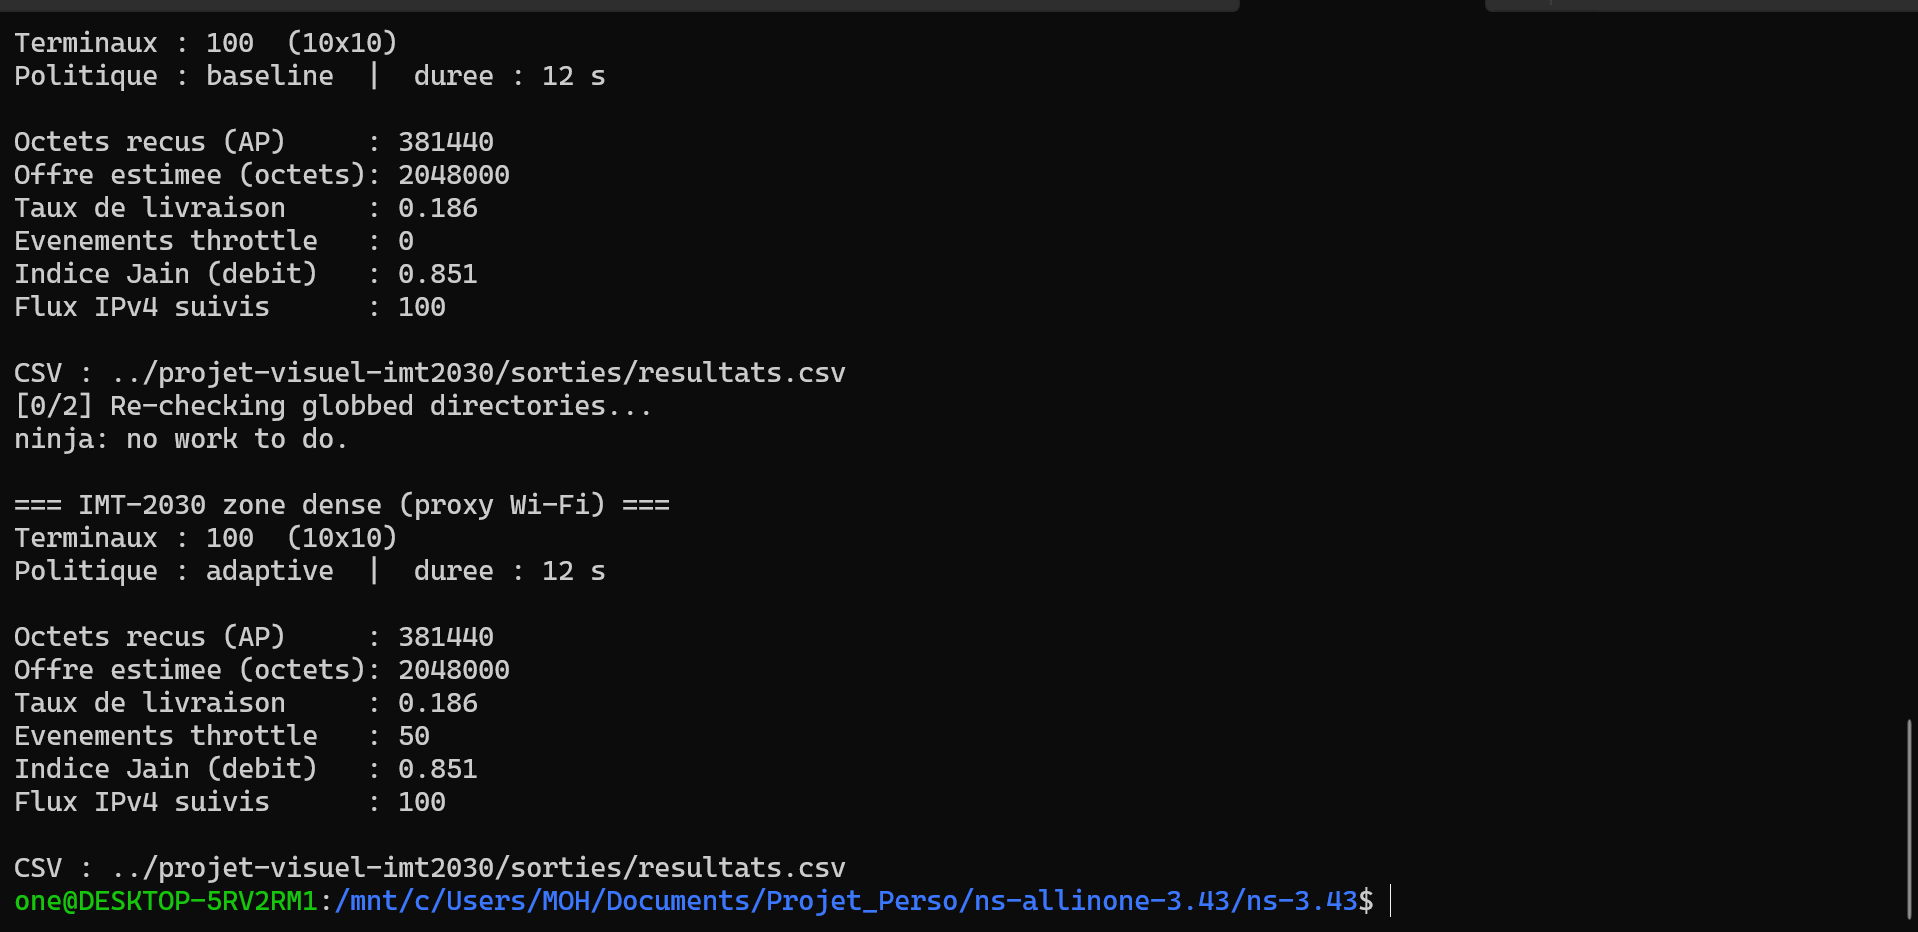
\includegraphics[width=0.95\linewidth]{../../labs/lab01_wifi_dense/docs/img/terminal-baseline-et-adaptive-10x10.png}
  \caption{Sortie terminal : baseline puis adaptive, même charge (\texttt{intervalMs=40}).}
\end{figure}

\section{Commandes de reproduction}

\begin{lstlisting}[language=bash]
cd /chemin/vers/ns-3.43
./ns3 build scratch/projet-visuel-imt2030/imt2030-density-gestion
./ns3 run "scratch/projet-visuel-imt2030/imt2030-density-gestion \
  --policy=baseline --gridSide=10 --simTime=12 --intervalMs=40"
./ns3 run "scratch/projet-visuel-imt2030/imt2030-density-gestion \
  --policy=adaptive --gridSide=10 --simTime=12 --intervalMs=40"
python3 labs/lab01_wifi_dense/scripts/generer_toutes_les_images.py
\end{lstlisting}

\section{Limites et suites planifiées}

Le Lab 1 fixe des positions constantes et une offre estimée à partir des paquets prévus. La capacité de référence est un paramètre analytique et non une mesure PHY directe. Le Lab 2 visera des campagnes systématiques, le Lab 3 une révision du contrôleur, le Lab 4 l'intégration 5G-LENA, et le Lab 5 une boucle de contrôle documentée de type AI-native.

\section{Compilation de ce rapport en PDF}

Depuis le dossier \texttt{docs/latex/}, sous WSL avec \texttt{texlive} installé~:

\begin{lstlisting}[language=bash]
cd docs/latex
pdflatex rapport_lab01.tex
pdflatex rapport_lab01.tex
\end{lstlisting}

Le fichier produit est \texttt{rapport\_lab01.pdf}. Si \texttt{pdflatex} ne charge pas les SVG, convertissez les figures en PNG ou commentez les trois figures \texttt{figure} avant compilation.

\end{document}
